En cumplimiento de lo dispuesto en el Decreto 1294 de 2021, el Convenio de Chicago de 1944 y el Reglamento Aeronáutico Colombiano RAC 100, Skyfilms, como explotador de Sistemas de Aeronaves No Tripuladas (UAS), en la Categoría Específica para operaciones de simple captura de imágenes o datos, emite la presente Declaración de Cumplimiento:

\begin{enumerate}
    \item Skyfilms manifiesta que su Sistema de Gestión de la Seguridad Operacional (SMS) y todas sus operaciones con UAS se desarrollan en estricto apego al RAC 100, al RAC 219 (incluidas las disposiciones de implementación del SMS, entre ellas la 219.105) y demás normas aeronáuticas vigentes en la República de Colombia.
    \item La empresa se compromete a implementar los procedimientos de este Manual de Seguridad Operacional y de los Manuales de Operaciones y de Control de Mantenimiento, para gestionar los riesgos, proteger a terceros y preservar la seguridad operacional en todas sus actividades.
    \item Se reconoce la autoridad de la Unidad Administrativa Especial de Aeronáutica Civil (Aerocivil) como ente regulador, certificador y supervisor de las operaciones aéreas con UAS en el territorio nacional.
    \item Skyfilms se obliga a mantener actualizada la información de este Manual y a informar y someter a aprobación de la Aerocivil sus revisiones y enmiendas, según el procedimiento del Control de Enmiendas y Revisiones.
    \item Todo el personal vinculado a Skyfilms S.A.S. está obligado a conocer y aplicar todos los procesos y procedimientos de este Manual de Seguridad Operacional, y el Ejecutivo Responsable se compromete a proveer los recursos para ello.
\end{enumerate}

\vspace{0.3cm}

\begin{center}

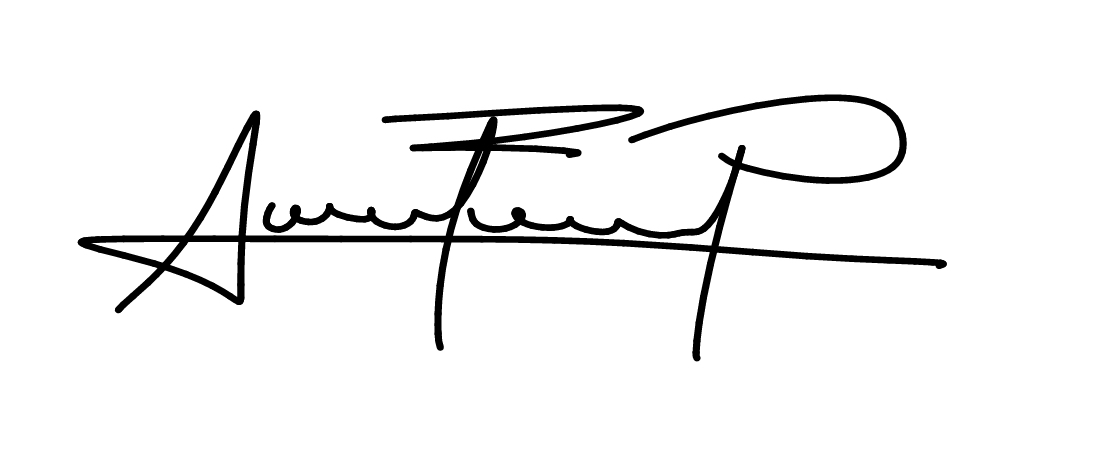
\includegraphics[width=4cm]{Imagenes/firma.jpg}

\vspace{-1.2cm}

\rule{7cm}{0.5pt}

\vspace{0.3cm}
\textbf{Andrés Felipe Pérez Sierra}\\
C.C. 1.108.206.142\\
Gerente General\\


\end{center}